\documentclass[10pt]{article}

\usepackage[T1]{fontenc}
\usepackage[left=2cm, right=2cm, top=2cm, bottom=2cm, paperheight=31cm]{geometry}
\usepackage[skins]{tcolorbox}
\usepackage{hyperref, fancyhdr, lastpage, tocloft, ragged2e, multicol, changepage}
\usepackage{amsmath, amssymb, amsthm, stmaryrd, calrsfs}
\usepackage{tkz-tab}
\usepackage{systeme}

\def\pagetitle{Relations Binaires}
\setlength{\headheight}{13pt}

\title{\bf{\pagetitle}\\\large{Corrigé}}
\date{Décembre 2023}
\author{DARVOUX Théo}

\DeclareMathOperator{\ch}{ch}

\hypersetup{
    colorlinks=true,
    citecolor=black,
    linktoc=all,
    linkcolor=blue
}

\pagestyle{fancy}
\cfoot{\thepage\ sur \pageref*{LastPage}}

\begin{document}
\renewcommand*\contentsname{Exercices.}
\renewcommand*{\cftsecleader}{\cftdotfill{\cftdotsep}}
\maketitle

\hrule
\tableofcontents
\vspace{0.5cm}
\hrule

\thispagestyle{fancy}
\fancyhead[L]{MP2I Paul Valéry}
\fancyhead[C]{\pagetitle}
\fancyhead[R]{2023-2024}
\allowdisplaybreaks

\pagebreak


\section*{Exercice 16.1 [$\blacklozenge\blacklozenge\lozenge$]}
\begin{tcolorbox}[enhanced, width=7.6in, center, size=fbox, fontupper=\large, drop shadow southwest]
    Soit $\mathcal{R}$ la relation définie sur $\mathbb{R}$ par :
    \begin{equation*}
        x ~\mathcal{R} ~ y \iff xe^y = ye^x.
    \end{equation*}
    1. Montrer que $\mathcal{R}$ est une relation d'équivalence sur $\mathbb{R}$.\\
    2. Préciser le cardinal de la classe d'équivalence d'un réel $x$.\\[0.1cm]
    1. Réflexivité : Soit $x\in\mathbb{R}$, on a bien que $xe^x = xe^x$.\\
    Symétrie : Soient $x,y\in\mathbb{R}$ tels que $xe^y = ye^x$, on a bien $ye^x = xe^y$.\\
    Transitivité : Soient $x,y,z\in\mathbb{R}$ tels que $xe^y = ye^x$ et $ye^z = ze^y$. Montrons que $xe^z = ze^x$.\\
    D'après la première égalité, $y=xe^{y-x}$.\\
    On remplace $y$ dans la seconde : $xe^{y-x+z}=ze^y$.\\
    On divise par $e^y$ : $xe^{z-x}=z$. On multiplie par $e^x$ : $xe^z = ze^x$.\\
    On a bien $x ~ \mathcal{R} ~ z$.\\[0.2cm]
    2. Soient $x,y\in\mathbb{R}$.\\
    On a $x ~ \mathcal{R} ~ y \iff \frac{x}{e^x} = \frac{y}{e^y}$.\\
    On pose $f:x\mapsto \frac{x}{e^x}$. La classe d'équivalence de $x$ est alors $\{y\in\mathbb{R} ~ | ~ f(x) = f(y)\}$.\\
    On a que $f$ est dérivable et $f':x\mapsto \frac{1-x}{e^{x}}$. Alors :
    \begin{center}
        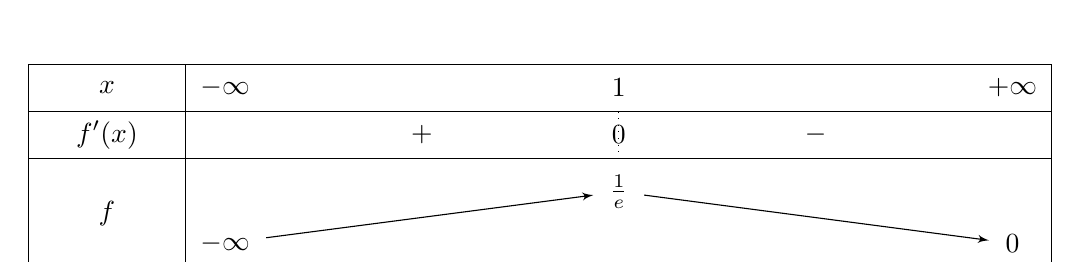
\begin{tikzpicture}
            \tkzTabInit[espcl=5]{$x$/0.6,$f'(x)$/0.6,$f$/1.4}{$-\infty$,$1$,$+\infty$}
            \tkzTabLine{,+,z,-,}
            \tkzTabVar{-/$-\infty$, +/$\frac{1}{e}$, -/$0$}
        \end{tikzpicture}
    \end{center}
    Alors, pour $x\in]-\infty,0]$, $|[x]|=1$, pour $x=1$, $|[x]|=1$ et sinon, $|[x]|=2$.\\
    \qed
\end{tcolorbox}
\addcontentsline{toc}{section}{\protect\numberline{}Exercice 16.1}


\end{document}
 
